\begin{frame}
    \small
    \frametitle{\begin{flushright}\textcolor{blue}{О}птимальная система счисления\end{flushright}}
    \begin{flushleft}
        \textbf{Задача}. Робинзон Крузо нашёл на острове 60 камней. Сколько прошедших дней можно ими закодировать в разных СС?
    \end{flushleft}
    \begin{minipage}{12.5cm}
        \raisebox{9\height}{\textbf{Пример СС-10}:}
        \hspace*{0.1in}
        \raisebox{0.02\height}{
\includegraphics[height=1in]{dots.png}}
        \hspace*{-0.1in}
        \raisebox{4\height}{
\includegraphics[height=13px]{arrow.png}}
        \hspace*{0in}
        \begin{minipage}{3.8cm}
            \footnotesize
            \raisebox{-1\height}{463502-й день из 999999 возможных,}
            \raisebox{-1\height}{где 999999 = 10$^{6}$ - 1}
            \raisebox{-1.1\height}{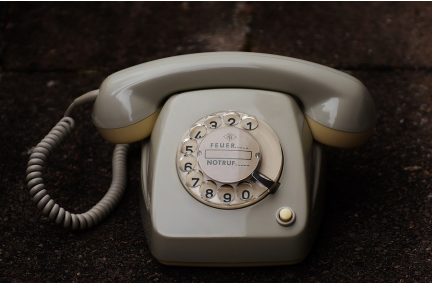
\includegraphics[height=100px]{phone.png}}
        \end{minipage}
    \end{minipage}
\end{frame}